%%%%%%%%%%%%%%%%%%%%%%%%%%%%%%%%%%%%%%%%%
% a0poster Portrait Poster
% LaTeX Template
% Version 1.0 (22/06/13)
%
% The a0poster class was created by:
% Gerlinde Kettl and Matthias Weiser (tex@kettl.de)
% 
% This template has been downloaded from:
% http://www.LaTeXTemplates.com
%
% License:
% CC BY-NC-SA 3.0 (http://creativecommons.org/licenses/by-nc-sa/3.0/)
%
%%%%%%%%%%%%%%%%%%%%%%%%%%%%%%%%%%%%%%%%%

%----------------------------------------------------------------------------------------
%	PACKAGES AND OTHER DOCUMENT CONFIGURATIONS
%----------------------------------------------------------------------------------------

\documentclass[a0,portrait]{a0poster}

\usepackage{multicol} % This is so we can have multiple columns of text side-by-side
\columnsep=100pt % This is the amount of white space between the columns in the poster
\columnseprule=3pt % This is the thickness of the black line between the columns in the poster

\usepackage[svgnames]{xcolor} % Specify colors by their 'svgnames', for a full list of all colors available see here: http://www.latextemplates.com/svgnames-colors

\usepackage{times} % Use the times font
%\usepackage{palatino} % Uncomment to use the Palatino font

\usepackage{graphicx} % Required for including images
\graphicspath{{figures/}} % Location of the graphics files
\usepackage{booktabs} % Top and bottom rules for table
\usepackage[font=small,labelfont=bf]{caption} % Required for specifying captions to tables and figures
\usepackage{amsfonts, amsmath, amsthm, amssymb} % For math fonts, symbols and environments
\usepackage{wrapfig} % Allows wrapping text around tables and figures

\begin{document}

%----------------------------------------------------------------------------------------
%	POSTER HEADER 
%----------------------------------------------------------------------------------------

% The header is divided into two boxes:
% The first is 75% wide and houses the title, subtitle, names, university/organization and contact information
% The second is 25% wide and houses a logo for your university/organization or a photo of you
% The widths of these boxes can be easily edited to accommodate your content as you see fit

\begin{minipage}[b]{0.75\linewidth}
\veryHuge \color{NavyBlue} \textbf{Fish recognition using deep convolutional neural network and data augmentation} \color{Black}\\ % Title
\Huge\textit{An Exploration of Complexity}\\[2cm] % Subtitle
\huge \textbf{Ziqiang Zheng}\\[0.5cm] % Author(s)
\huge Ocean University of China\\[0.4cm] % University/organization
\Large \texttt{zhengziqiang1@gmail.com}\\
\end{minipage}
%
\begin{minipage}[b]{0.25\linewidth}
\includegraphics[width=20cm]{ouc.jpg}\\
\end{minipage}

\vspace{1cm} % A bit of extra whitespace between the header and poster content

%----------------------------------------------------------------------------------------

\begin{multicols}{2} % This is how many columns your poster will be broken into, a portrait poster is generally split into 2 columns

%----------------------------------------------------------------------------------------
%	ABSTRACT
%----------------------------------------------------------------------------------------

\color{Navy} % Navy color for the abstract

\begin{abstract}

Nowadays, as a sub topic of computer vision and fishery industry, fish recognition is still a challenging work not only because of various kinds of fish, but also because of the complex background of images. In this paper, we aim to classify different fish images obtained from cameras of fishing vessels. Fish detection is different with the best known and the most well-investigated object detection - face detection. Fish has more different shapes than human faces. And fish always take only a small part of the whole image. For these two reasons, it's a challenge for us to detect and classify the fish. Our work is done with Kaggle dataset. The Kaggle dataset aims to detect and classify the species of fish. The competition provides a train dataset which contains six species of tuna fish, fish but not tuna and no fish. Eight target categories are available in the dataset. The dataset is critically imbalanced, the Albacore tuna has thousands of images while the Opah has only sixty images. In order to overcome these problems we introduced two methods to improve our accuracy for the fish classification. Our approach can avoid over-fitting caused by the imbalance of training dataset. We employ the AlexNet, GoogLeNet, Caffenet and VGGNet neural network for the classification. As a result of the small dataset, the VGGNet architecture performs worse than AlexNet. We propose a local region based the fish area modeling approach so that the local feature can be modeled. In order to obtain more image information and realize imbalanced datasets classification, we have done some data augmentation. In order to get better performance, we also have done some image preprocessing, and it really works.

\end{abstract}

%----------------------------------------------------------------------------------------
%	INTRODUCTION
%----------------------------------------------------------------------------------------

\color{SaddleBrown} % SaddleBrown color for the introduction

\section*{Introduction}
In this paper, we will introduce two methods to improve the classification accuracy. Our methods can be described with the Fig.~\ref{fig:process}. We have done some data preprocessing before training our model. First we make a mask in the fish region and make the fish region black, which we regard as the NoF fish images. Then we use some methods to achieve data augmentation. At last we use the convolutional neural network(CNN) as the classifier. The first method is based on data augmentation. In consideration of the imbalance of the dataset, we got some new images by rotating the selected images. Through this method, we can increase the number of some species of fish images, which can help avoid that our model is over-fitted with some categories of fish images, and rotating the fish images can improve the robustness of detection and achieve sophisticated detection. We increased the size of our datasets in this way and the validation accuracy increased two percent.



%----------------------------------------------------------------------------------------
%	OBJECTIVES
%----------------------------------------------------------------------------------------

\color{DarkSlateGray} % DarkSlateGray color for the rest of the content

\section*{Main Objectives}

\begin{enumerate}
\item First we make a mask of the fish region.
\item Nullam at mi nisl. Vestibulum est purus, ultricies cursus volutpat sit amet, vestibulum eu.
\item Praesent tortor libero, vulputate quis elementum a, iaculis.
\item Phasellus a quam mauris, non varius mauris. Fusce tristique, enim tempor varius porta, elit purus commodo velit, pretium mattis ligula nisl nec ante.
\item Ut adipiscing accumsan sapien, sit amet pretium.
\item Estibulum est purus, ultricies cursus volutpat
\item Nullam at mi nisl. Vestibulum est purus, ultricies cursus volutpat sit amet, vestibulum eu.
\item Praesent tortor libero, vulputate quis elementum a, iaculis.
\end{enumerate}

%----------------------------------------------------------------------------------------
%	MATERIALS AND METHODS
%----------------------------------------------------------------------------------------

\section*{Methods}

Fusce magna risus, molestie ut porttitor in, consectetur sed mi. Vestibulum ante ipsum primis in faucibus orci luctus et ultrices posuere cubilia Curae; Pellentesque consectetur blandit pellentesque. Sed odio justo, viverra nec porttitor vel, lacinia a nunc. Suspendisse pulvinar euismod arcu, sit amet accumsan enim fermentum quis. In id mauris ut dui feugiat egestas. Vestibulum ac turpis lacinia nisl commodo sagittis eget sit amet sapien.

%------------------------------------------------



\section*{Results}

Donec faucibus purus at tortor egestas eu fermentum dolor facilisis. Maecenas tempor dui eu neque fringilla rutrum. Mauris \emph{lobortis} nisl accumsan. Aenean vitae risus ante.
%
\begin{wraptable}{l}{12cm} % Left or right alignment is specified in the first bracket, the width of the table is in the second
\begin{tabular}{l l l}
\toprule
\textbf{Database} & \textbf{Model} & \textbf{Accuracy}\\
\midrule
       full+rotating & alexnet     & 0.9673  \\
       full+rotating & googlenet   &0.964    \\
       full+rotating  & vgg16  & 0.45  \\
\bottomrule
\end{tabular}
\captionof{table}{\color{Green} The validation accuracy in Kaggle database}
\end{wraptable}
%
Phasellus imperdiet, tortor vitae congue bibendum, felis enim sagittis lorem, et volutpat ante orci sagittis mi. Morbi rutrum laoreet semper. Morbi accumsan enim nec tortor consectetur non commodo nisi sollicitudin. Proin sollicitudin. Pellentesque eget orci eros. Fusce ultricies, tellus et pellentesque fringilla, ante massa luctus libero, quis tristique purus urna nec nibh.

Nulla ut porttitor enim. Suspendisse venenatis dui eget eros gravida tempor. Mauris feugiat elit et augue placerat ultrices. Morbi accumsan enim nec tortor consectetur non commodo. Pellentesque condimentum dui. Etiam sagittis purus non tellus tempor volutpat. Donec et dui non massa tristique adipiscing. Quisque vestibulum eros eu. Phasellus imperdiet, tortor vitae congue bibendum, felis enim sagittis lorem, et volutpat ante orci sagittis mi. Morbi rutrum laoreet semper. Morbi accumsan enim nec tortor consectetur non commodo nisi sollicitudin.

\begin{center}\vspace{1cm}
\includegraphics[width=0.8\linewidth]{process}
\captionof{figure}{\color{Green} First we make a mask in the fish region, then we rotate the processed images at different angles and get some new different images. After the data augmentation, at last we use the CNN to fish the fish classification.}
\end{center}\vspace{1cm}

In hac habitasse platea dictumst. Etiam placerat, risus ac.

Adipiscing lectus in magna blandit:

\begin{center}\vspace{1cm}
\begin{tabular}{l l l l}
\toprule
\textbf{Method} & \textbf{Model} & \textbf{Test loss} \\
\midrule
	None	& Caffenet	& 1.92 \\
       None	& GoogleNet	& 2.56 \\
       Rotating & Caffenet     & 1.77  \\
       Rotating & GoogleNet   & 1.93    \\
	Mask	& Caffenet	& 1.87   \\
	Mask	& GoogleNet	& 2.25    \\
	Rotating + Mask &Caffenet & 1.71   \\
	Rotating + Mask &GoogleNet & 1.85  \\
\bottomrule
\end{tabular}
\captionof{table}{\color{Green} The test loss in the Kaggle competition}
\end{center}\vspace{1cm}

Vivamus sed nibh ac metus tristique tristique a vitae ante. Sed lobortis mi ut arcu fringilla et adipiscing ligula rutrum. Aenean turpis velit, placerat eget tincidunt nec, ornare in nisl. In placerat.

\begin{center}\vspace{1cm}
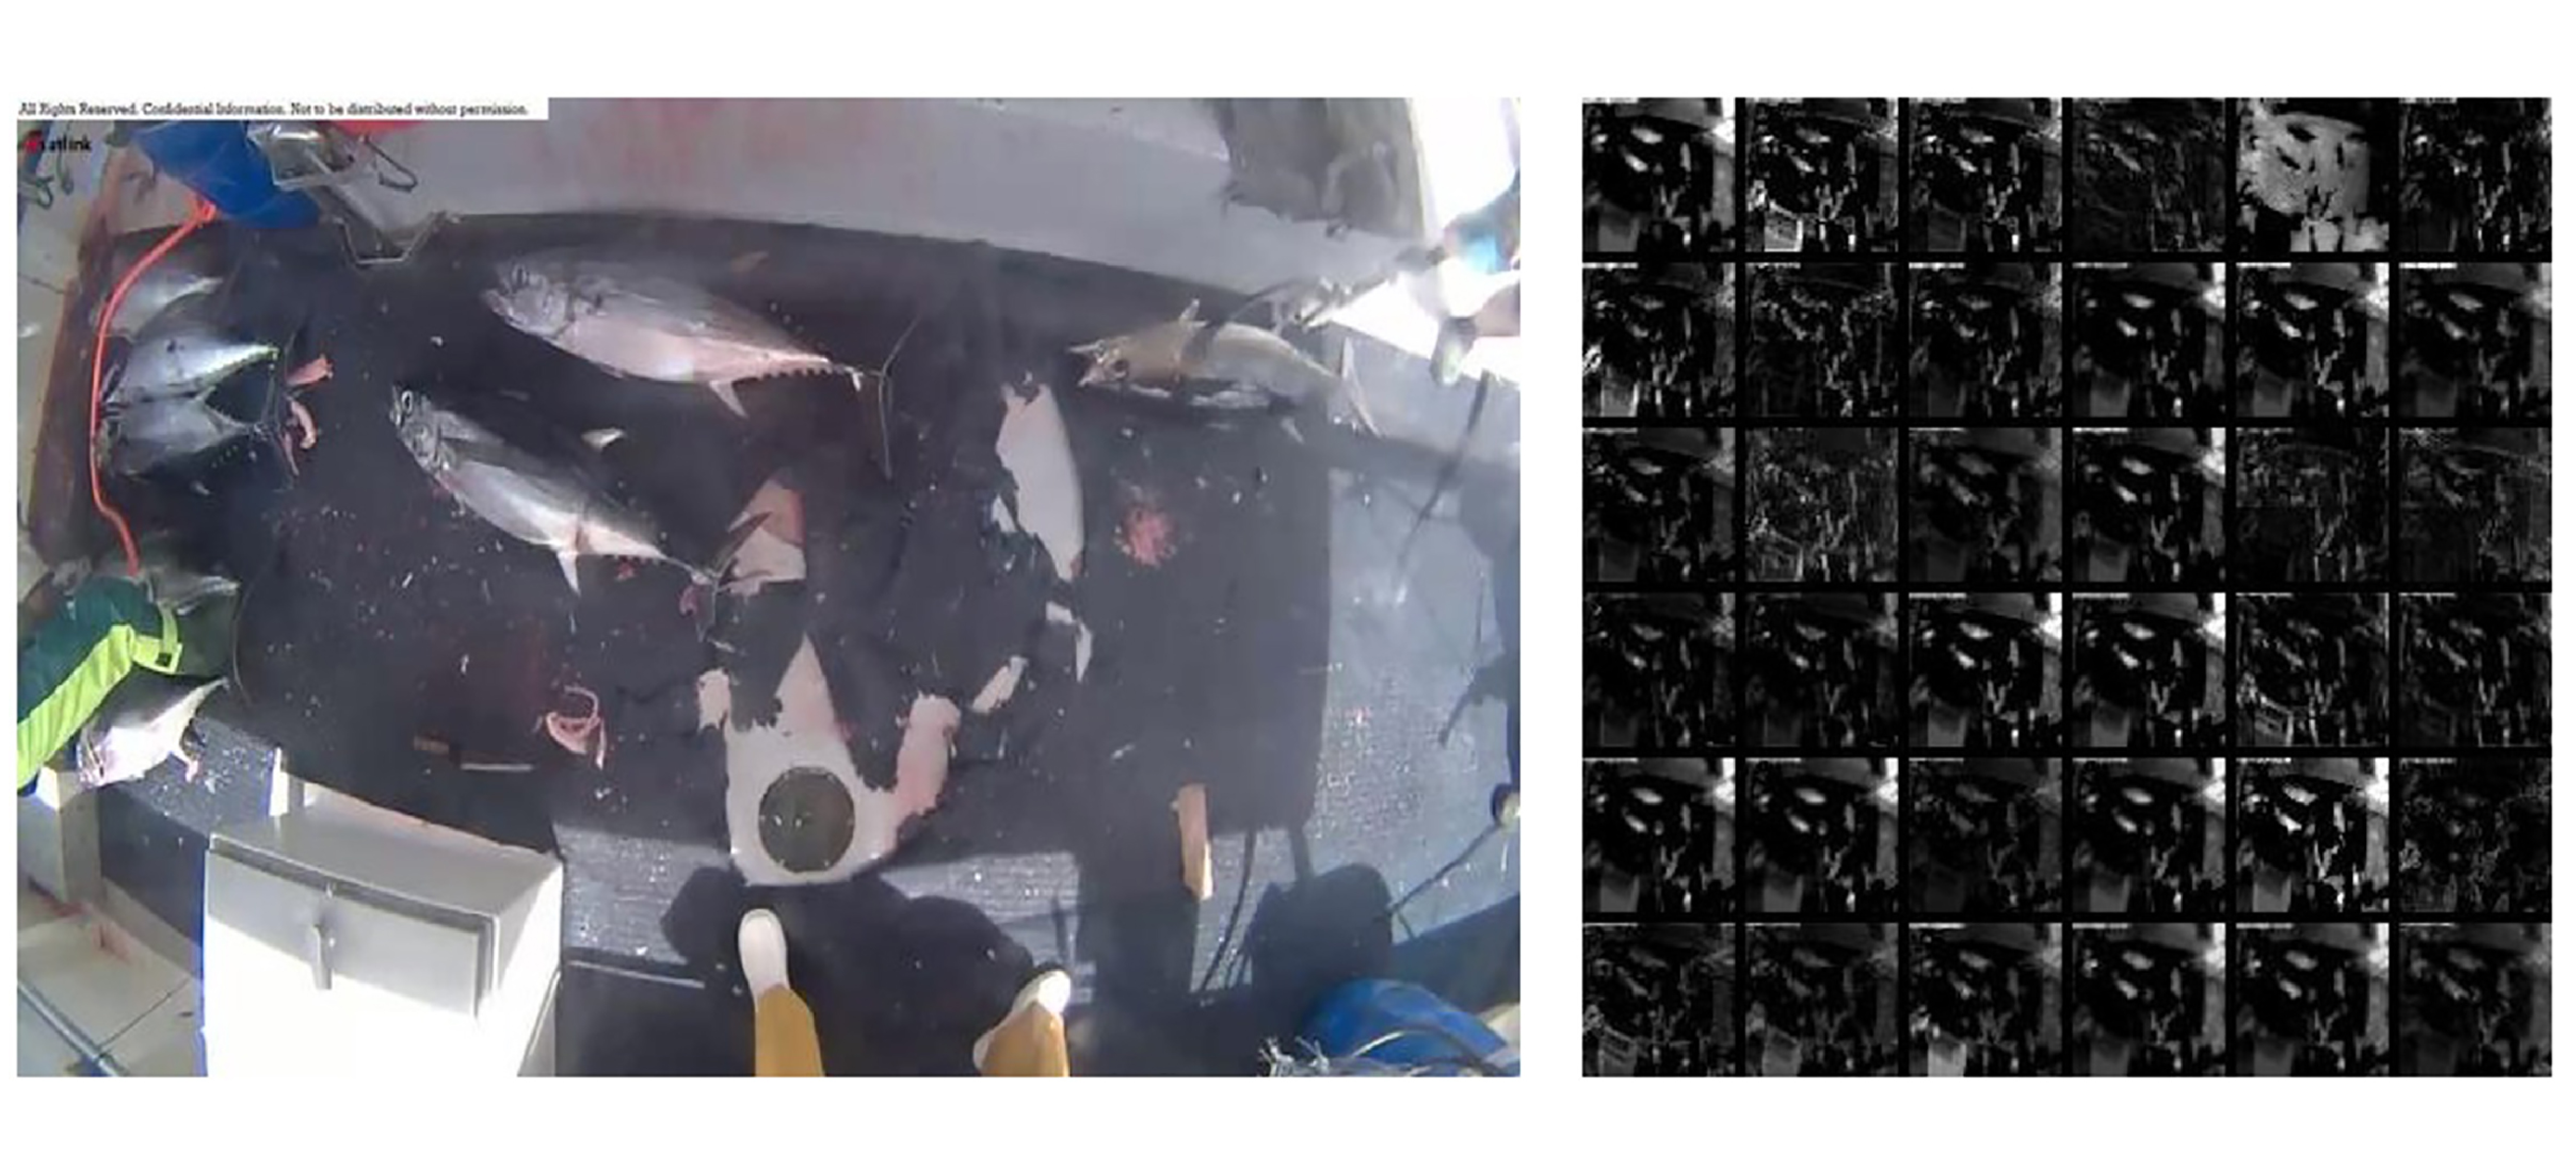
\includegraphics[width=0.8\linewidth]{merge}
\captionof{figure}{\color{Green} There are 36 pooling images in the final pooling image. Considering that the size of the pooling images and the number of them, we make them smaller by resizing the images and merge them into one image. By comparing the two images, The region of fish are brighter than other regions in the most of the pooling images, which can prove that the fish has more influence on the classification than other regions.}
\end{center}\vspace{1cm}

%----------------------------------------------------------------------------------------
%	CONCLUSIONS
%----------------------------------------------------------------------------------------

\color{SaddleBrown} % SaddleBrown color for the conclusions to make them stand out

\section*{Conclusions}

\begin{itemize}
\item The two methods we have used improved the deep neural networks to detect the fish more efficiently.
\item The image processing methods such as rotating and making mask can also work to get the better performance.
\item Data augmentation methods can solve the imbalance of the dataset well and it can also improve the accuracy of our model..
\end{itemize}

\color{DarkSlateGray} % Set the color back to DarkSlateGray for the rest of the content

%----------------------------------------------------------------------------------------
%	FORTHCOMING RESEARCH
%----------------------------------------------------------------------------------------


 %----------------------------------------------------------------------------------------
%	REFERENCES
%----------------------------------------------------------------------------------------

\nocite{*} % Print all references regardless of whether they were cited in the poster or not
\bibliographystyle{plain} % Plain referencing style
\bibliography{sample} % Use the example bibliography file sample.bib

%----------------------------------------------------------------------------------------
%	ACKNOWLEDGEMENTS
%----------------------------------------------------------------------------------------



%----------------------------------------------------------------------------------------

\end{multicols}
\end{document}
